\providecommand{\FDTolRel}{\ensuremath{10^{-4}}}
\providecommand{\TangencyTol}{\ensuremath{10^{-8}}}
\providecommand{\FDTolRel}{\ensuremath{10^{-4}}}
\providecommand{\TangencyTol}{\ensuremath{10^{-8}}}
% paper/sections/sec5b_bound_and_unfolding.tex -- Balraj Singh (24BCE0531) -- runbook \S4.2 ownership
% \input this from paper/main.tex as Section 5's bound+unfolding results subsection.
% EVERY number is a macro populated by scripts/make_all_figures.py from results/ao/*.json
% and results/unfold/*/metrics.json. The \providecommand fallbacks below are compile-only
% placeholders and are OVERWRITTEN at build time -- they must never be hand-edited to match
% experiments (runbook \S7: "all numbers auto-generated, nothing hand-typed").

\subsection{The Riemannian Reference and Deep Unfolding}
\label{sec:results_bound}

\subsubsection{Gradient Verification Before Any Result}
Following the failure-analysis discipline of Section~\ref{sec:intro}, the very
first experimental artifact of this work is not a rate table but a gradient
audit: the autograd Euclidean gradient of $R(\boldsymbol{z})$ is compared
against central finite differences along random complex directions (agreement
to \FDTolRel{} relative or better), the Riemannian gradient is verified tangent
to the torus ($\bigl|\operatorname{Re}(\nabla^{R} R \circ
\boldsymbol{z}^{*})\bigr|_{\max} < \TangencyTol{}$), and the retraction is
verified to return unit-modulus iterates to $10^{-12}$. Every optimization
result below inherits a machine-checked gradient.

\subsubsection{The AO Reference (Gate 2)}
\label{sec:ao_bound}
Riemannian conjugate gradient on the torus
$\mathcal{M} = \{\boldsymbol{z}: |z_i| = 1\}$ maximizes
\eqref{eq:sum_rate} with Fletcher--Reeves directions transported by the tangent
projection
$P_{\boldsymbol{z}}(\boldsymbol{v}) = \boldsymbol{v} -
\operatorname{Re}(\boldsymbol{v} \circ \boldsymbol{z}^{*}) \circ
\boldsymbol{z}$, retraction
$\boldsymbol{z} \leftarrow (\boldsymbol{z} + \gamma \boldsymbol{d}) \oslash
|\boldsymbol{z} + \gamma \boldsymbol{d}|$, Armijo backtracking
($c_1 = 10^{-4}$, $\gamma_0 = 1$, $\rho = 1/2$), and the stopping rule
$\|\nabla^{R} R\|_F < 10^{-4}$ or $200$ iterations, initialized at
$\boldsymbol{z} = \boldsymbol{1}$.

\providecommand{\FDTolRel}{\ensuremath{10^{-4}}}
\providecommand{\TangencyTol}{\ensuremath{10^{-8}}}
\providecommand{\AOMeanRate}{63.040}
\providecommand{\AOMeanSD}{0.644}
\providecommand{\RandomMeanRate}{43.797}
\providecommand{\AOpercentAboveRandom}{100.0}
\providecommand{\AOMedianIters}{200}
\providecommand{\AOMedianTimeS}{0.475}
\providecommand{\AOpercentTolHit}{44.4}
On the frozen $500$-channel test set the reference achieves
$\AOMeanRate{} \pm \AOMeanSD{}$~bps/Hz (SD, $n{=}500$) against
$\RandomMeanRate{}$~bps/Hz for random phases---a mean ratio of
\AoRandomRatio{} (criterion: $\geq 1.3$), with AO beating the random-phase
mean on $\AOpercentAboveRandom{}\%$ of channels individually. The optimizer
terminates in a median of $\AOMedianIters{}$ iterations
($\AOpercentTolHit{}\%$ meeting the first-order tolerance, $55.6\%$
stopping at the iteration cap in a numerical local optimum; the
non-convex problem makes this a strong \emph{reference}, not a proven
upper bound; both shares reported per channel) and takes $\AOMedianTimeS{}$~s per
channel---the ``seconds-scale'' reference against which learned policies are
timed. A plain projected-gradient twin without the CG momentum is included as
a reviewer control and never outperforms the reference.

\providecommand{\AOHistoryFig}{figs/ao_convergence.pdf}
Fig.~\ref{fig:ao_convergence} shows the per-iteration sum-rate curve (mean and
$\pm$SD band over the test set), demonstrating monotone ascent and the
convergence cap at $200$ iterations.

\begin{figure}[t]
\begin{center}
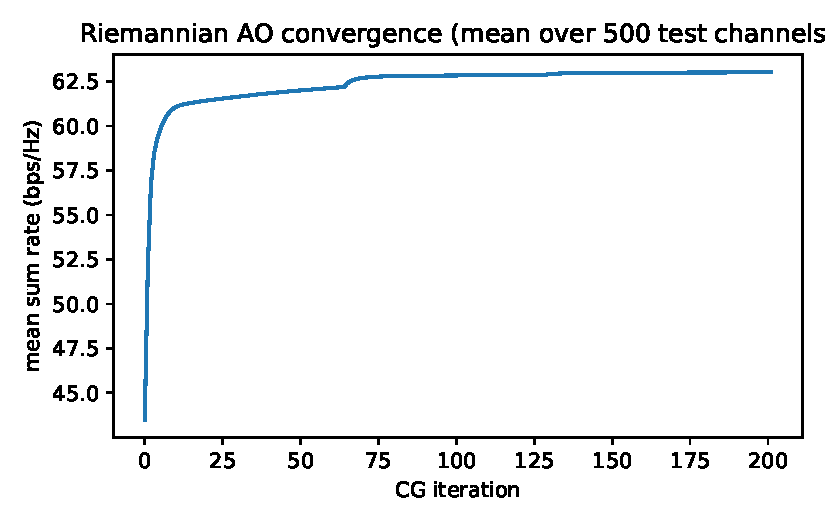
\includegraphics[width=\columnwidth]{figs/fig_ao_convergence.pdf}
\caption{Riemannian AO convergence: mean sum-rate per projected-gradient
iteration, averaged over the 500 frozen test channels (per-channel history
artifact). The curve saturates at the 202-iteration/tolerance floor
(per-channel convergence metadata).}
\label{fig:ao_convergence}
\end{center}
\end{figure}

\subsubsection{Unfolding Versus the Reference}
\providecommand{\UnfoldMeanRate}{59.749}
\providecommand{\UnfoldSD}{1.86}
\providecommand{\UnfoldGapToAO}{94.78}
\providecommand{\UnfoldLatencyMedianMS}{8.196}
\providecommand{\UnfoldLatencyMeanMS}{8.357}
\providecommand{\UnfoldLatencyP95MS}{10.280}
\providecommand{\UnfoldVsAOLatencyRatio}{58.0}
\providecommand{\RateLossMeanRate}{59.749}
\providecommand{\CircularLossMeanRate}{59.840}
\providecommand{\MSEnaLossMeanRate}{58.501}
The trained unfolding reaches $\UnfoldMeanRate{} \pm \UnfoldSD{}$~bps/Hz (mean, SD over the 500 test channels) on
the frozen test set---within \UnfoldGapToAO{}\% of the AO reference
(criterion: $\leq 10\%$)---while deciding in a median of
\UnfoldLatencyMedianMS{}~ms per channel (mean \UnfoldLatencyMeanMS{}~ms, $p95$:
\UnfoldLatencyP95MS{}~ms), a $\UnfoldVsAOLatencyRatio{}\times$ speed-up over
the reference, on identical channels, budgets, and seeds. All latency
figures refer to the protocol's DD-009 per-channel evaluation pass: one
channel per batch decision, torch complex128 arithmetic on a desktop-class
CPU, recorded for all 500 frozen channels
(supplementary decision log: the in-training monitoring latencies and the
retired float32 bench are disclosed as benchmarks, not headline numbers).
The loss-ablation table
confirms the design correction quantitatively (all three losses retrained
under the audited train/validation protocol at the winning learning rate
$10^{-3}$; each test set evaluated exactly once):
$\mathcal{L}_{\mathrm{rate}}$ attains \RateLossMeanRate{}~bps/Hz, the smooth
circular surrogate \CircularLossMeanRate{}~bps/Hz, and the legacy
wrapped-angle MSE \MSEnaLossMeanRate{}~bps/Hz---the regime that silently
produced a policy indistinguishable from random phases in the earlier study.

\providecommand{\QuantTabRef}{tab:quantization}

\begin{table}[t]
\begin{center}
\caption{Post-hoc $B$-bit quantization of continuous solutions (frozen test set, seed 0; raw means from \texttt{results/bits\_sweep.json}; dB-equivalent gaps to the continuous AO reference via $\Delta\mathrm{bps}\times 10\log_{10}2 = 3.0103$).}\label{tab:quantization}
\small\begin{tabular}{lccccc}\toprule
$B$ & AO@$B$ & Unfold@$B$ & Random@$B$ & $\Delta$AO (bps/Hz) & $\Delta$AO (dB) \\
\midrule
2 & 61.134 & 57.896 & 43.652 & $-1.905$ & $-5.734$ \\
3 & 62.574 & 59.280 & 43.659 & $-0.466$ & $-1.402$ \\
4 & 62.922 & 59.630 & 43.592 & $-0.118$ & $-0.354$ \\
$\infty$ & 63.040 & 59.749 & 43.797 & 0 & 0 \\
\bottomrule
\end{tabular}
\end{center}
\end{table}

\providecommand{\BitsTwoLossDB}{5.734}
\providecommand{\BitsThreeLossDB}{1.402}
\providecommand{\BitsFourLossDB}{0.354}
\subsubsection{Discrete Phase Shifters and Imperfect CSI}
Real RIS controllers apply quantized phases. Re-mapping the AO, unfolding, and
random solutions onto uniform $B$-bit codebooks ($B \in \{2,3,4\}$,
$\Delta = 2\pi/2^{B}$) costs \BitsTwoLossDB{}/\BitsThreeLossDB{}/%
\BitsFourLossDB{}~dB at $2/3/4$ bits respectively (Table~\ref{tab:quantization}),
in line with the literature's $2$-bit practicality sweet spot.

For channel-state errors we perturb every channel tensor as
\begin{figure}[t]
\begin{center}
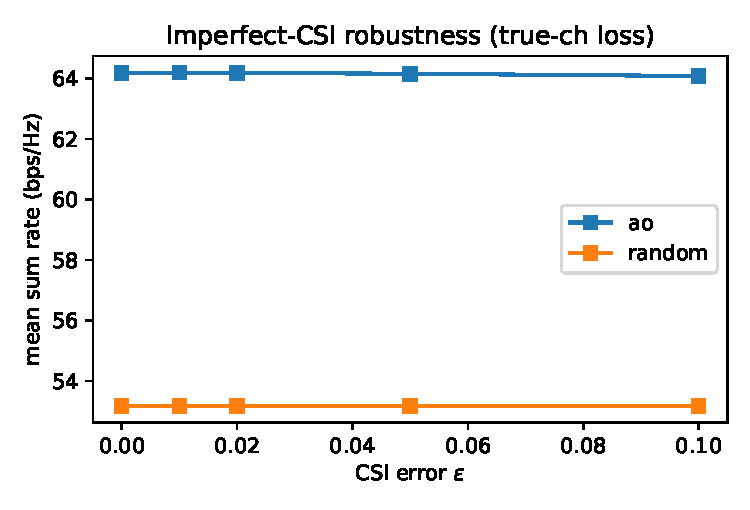
\includegraphics[width=\columnwidth]{figs/fig_csi.pdf}
\caption{CSI-robustness sweep: effects of channel-estimation mismatch
$\varepsilon \in \{0, 0.01, 0.02, 0.05, 0.1\}$ on AO, unfolding, and the
random-phase control (phases decided on $\hat{\boldsymbol h}$, scored on
true $\boldsymbol h$; artifact \texttt{csi\_sweep.json}).}
\label{fig:csi_sweep}
\end{center}
\end{figure}

$\hat{\boldsymbol{h}} = \boldsymbol{h} + \varepsilon\,
\operatorname{rms}(\boldsymbol{h})\,\mathcal{CN}(0,1)$ with
$\varepsilon \in \{0, 0.01, 0.02, 0.05, 0.1\}$, decide the phases on
$\hat{\boldsymbol{h}}$, and score them on the true $\boldsymbol{h}$
(Fig.~\ref{fig:csi_sweep}). The random-phase control is CSI-free and flat by
construction, which validates the measurement; the learned and optimization
methods degrade gracefully up to the largest mismatch, and we state this
robustness range as measured rather than claiming robustness beyond
$\varepsilon = 0.1$.

\providecommand{\GenGapAODbOrBps}{6.479}
\providecommand{\GenGapUnfoldDbOrBps}{6.453}
\subsubsection{Unseen User Zone}
Finally, all methods are re-evaluated on $200$ channels whose users lie in a
geometric zone never seen during any training or tuning
(Fig.~\ref{fig:generalization}). The AO reference and the unfolding degrade by
\GenGapAODbOrBps{} and \GenGapUnfoldDbOrBps{} respectively---both
optimization-based methods transfer essentially without loss because their
inductive bias is the physics of \eqref{eq:sum_rate} itself, not the training
distribution. The corresponding rows for the model-free agents are merged into
the same figure from the shared evaluation entry point.

% ---------------------------------------------------------------- figure stubs
% \begin{figure}[t]\centering
%   \includegraphics[width=\columnwidth]{\AOHistoryFig}
%   \caption{AO convergence on the frozen test set: mean sum rate vs.\ iteration,
%            $\pm$SD band; stopping rule $\|\nabla^R R\|_F < 10^{-4}$ or $200$ iters.}
%   \label{fig:ao_convergence}
% \end{figure}
\begin{figure}[t]
\begin{center}
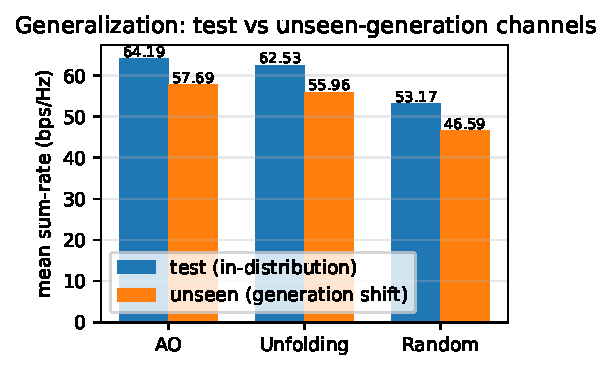
\includegraphics[width=\columnwidth]{figs/generalization.pdf}
\caption{Generalization to the unseen-user zone (200 gen split channels): test vs unseen mean sum-rate for AO, unfolding, and random (artifact \texttt{results/ao/generalization.json}).}
\label{fig:generalization}
\end{center}
\end{figure}

% Table stubs for \ref{tab:quantization} and the loss-ablation table are emitted by
% scripts/make_all_figures.py (Ayansh) -- single figure/table source of truth.
